\documentclass{sigchi}

% Use this command to override the default ACM copyright statement
% (e.g. for preprints).  Consult the conference website for the
% camera-ready copyright statement.


%% BEGIN -- OVERRIDE THE DEFAULT COPYRIGHT STRIP
\toappear{
    This work is licensed under the Creative Commons Attribution-ShareAlike
    4.0 International License. To view a copy of this license, visit\\
    {\url{http://creativecommons.org/licenses/by-sa/4.0/}}.
    {Copyright \copyright~2015 Authors}}
%% END -- OVERRIDE THE DEFAULT COPYRIGHT STRIP


% Arabic page numbers for submission.  Remove this line to eliminate
% page numbers for the camera ready copy

%\pagenumbering{arabic}

% Load basic packages
\usepackage{balance}  % to better equalize the last page
\usepackage{graphics} % for EPS, load graphicx instead
%\usepackage[T1]{fontenc}
\usepackage{txfonts}
\usepackage{times}    % comment if you want LaTeX's default font
\usepackage[pdftex]{hyperref}
% \usepackage{url}      % llt: nicely formatted URLs
\usepackage{color}
\usepackage{textcomp}
\usepackage{booktabs}
\usepackage{ccicons}
\usepackage{todonotes}
\usepackage{footnote}
\usepackage{mathptmx,helvet,courier}  \usepackage{array}
\usepackage{ragged2e}
\usepackage{tabularx,ragged2e,booktabs,caption}
\newcolumntype{C}[1]{>{\Centering}m{#1}}
\renewcommand\tabularxcolumn[1]{C{#1}}
\usepackage{tablefootnote}
\usepackage{array}
\newcolumntype{P}[1]{>{\centering\arraybackslash}p{#1}}
\pagenumbering{arabic}
% llt: Define a global style for URLs, rather that the default one
\makeatletter
\def\url@leostyle{%
  \@ifundefined{selectfont}{\def\UrlFont{\sf}}{\def\UrlFont{\small\bf\ttfamily}}}
\makeatother
\urlstyle{leo}

% To make various LaTeX processors do the right thing with page size.
\def\pprw{8.5in}
\def\pprh{11in}
\special{papersize=\pprw,\pprh}
\setlength{\paperwidth}{\pprw}
\setlength{\paperheight}{\pprh}
\setlength{\pdfpagewidth}{\pprw}
\setlength{\pdfpageheight}{\pprh}

% Make sure hyperref comes last of your loaded packages, to give it a
% fighting chance of not being over-written, since its job is to
% redefine many LaTeX commands.
\definecolor{linkColor}{RGB}{6,125,233}
\hypersetup{%
    pdftitle={document},
    pdfauthor={},
    pdfkeywords={},
    bookmarksnumbered,
    pdfstartview={FitH},
    colorlinks,
    citecolor=black,
    filecolor=black,
    linkcolor=black,
    urlcolor=linkColor,
    breaklinks=true,
}

% create a shortcut to typeset table headings
% \newcommand\tabhead[1]{\small\textbf{#1}}

% End of preamble. Here it comes the document.
\begin{document}

\title{Extending StackOverflow® Gamification Using Social Media}

\numberofauthors{5}
\author{%
    \alignauthor{Arturo Reyes Lopez\\
        \affaddr{University of Victoria}\\
        \affaddr{Victoria, BC, Canada}\\
        \email{areyeslo@uvic.ca}}\\
    \alignauthor{Nitin Goyal\\
        \affaddr{University of Victoria}\\
        \affaddr{Victoria, BC, Canada}\\
        \email{ngoyal@uvic.ca}}\\
    \alignauthor{Richard B. Wagner\\
        \affaddr{University of Victoria}\\
        \affaddr{Victoria, BC, Canada}\\
        \email{rbwagner@uvic.ca}}\\
    \alignauthor{Tim Baker\\
        \affaddr{University of Victoria}\\
        \affaddr{Victoria, BC, Canada}\\
        \email{timbaker@uvic.ca}}\\
    \alignauthor{Alastair Beaumont\\
        \affaddr{University of Victoria}\\
        \affaddr{Victoria, BC, Canada}\\
        \email{alastair@uvic.ca}}\\
}

\maketitle

\begin{abstract}
Gamification is the application of game playing elements (point scoring, competition, badges etc.) to other areas of activity to encourage engagement and participation. StackOverflow is a popular Q\&A community, with thousands of users solving and answering questions. SO community uses elements of badges and reputation to practice gamification.  Our motivation for this project is to identify the effectiveness of gamification and how it can be improved further.We argued that inclusion of social media and classification of badges according to technical proficiencies could improve gamification.To conduct the qualitative analysis we used surveys and interviews.First group of users for the survey was a measured sample from SO community based on the reputation levels and the second group was from UVic students.Interviews are then conducted for users belonging to different reputation levels. Analysis from the survey results and interviews shows that inclusion of social media and technical proficiency is not required. However there is a need to from the end of SO community to reinforce the standards for earning badges and making the community inclusive for new users to foster contribution and collaboration.
\end{abstract}


\keywords{Gamification, StackOverflow (SO)}

\category{H.5.m.}{Information Interfaces and Presentation
  (e.g. HCI)}{Miscellaneous} \category{See
  \url{http://acm.org/about/class/1998/} for the full list of ACM
  classifiers. This section is required.}{}{}

\section{Introduction}
In Social Media, the use of game design and game elements, known as gamification, has sought to increase generation of content by the users. Badges, privileges and reputation are being used to recognize contributions of users on the sites and generally these elements seem to be valued by users who compete for some form of reward, be it monetary, building a reputation, recognition of skills, etc. Several studies have shown awareness of other participants and competence during the game experiences\cite{Rughinis}. Other studies have shown that gamification can increase engagement in activities that involve a community \cite{Marder}. However, the inclusion of gamification itself does not guarantee an increase in engagement or motivation and its effectiveness depends on the rules to earn badges and privileges  according to the context\cite{Deterding}.
StackOverflow (SO) is a popular Q\&A website for an ever-increasing range of computer programming topics. SO is likely to be the most popular website in the computer programming world with over 4,000,000 registered users \footnote{https://stackoverflow.com/users} and with more than 11,000,000 questions \footnote{https://stackoverflow.com/questions}. The website serves as a platform for users to both ask questions related to programming and to answer the questions of other users. These contributions by the users are the heart of the content and are met with reputation points and “badges” for the user. Our intention is to examine whether this use of gamification elements is a primary motivating factor for the users collaboration and if so, is it possible to improve the current system in order to foster an increase in collaboration by users that wouldn't normally contribute to the site? 
This research aims to examine the ways that collaboration, in the form of asking and answering questions and commenting on the questions, is achieved in SO and what changes can be made to encourage this kind of collaboration from more users and to promote an increase in contributions from users of all skill levels. 
While we are conducting our research, we are hoping to uncover sufficient evidence to affirm or negate our hypotheses on this subject. We would like to see whether there needs to be improvements made to the existing forms of gamification. As well, we hope to determine whether users would like to have the option to share their progress and achievements on social media platforms and if so, how and where would they like to be able to share it.
Throughout the course of this research, we will present an overview of relevant, related work, examine what the primary motivating factors are for user collaboration, discuss the merits and shortcomings of the current system, and provide our recommendations of how StackOverflow may be improved upon to encourage more active participation from a wider range of its users. 

\section{Related work}
StackOverflow has been heavily studied in recent years. The following section provides an insight into some related articles to our research questions.

The vast majority of StackOverflow users only post once. These "One-day flies on StackOverflow" are seen as a nuisance by other users as they do not provide to the website or 'upvote' the users that answer their questions. \cite{Slag} These users are more likely to not have their questions answered because the new users tend to ignore to person who answered their question by not providing them with reputation (by upvoting). New users are also more likely to recieve negative feedback or answers that can be interpreted that way because of this. This causes a gap between new users and the other more experienced users because of this view that new users will not contribute and creates a negative and unfriendly communitee to newcomers. This lack of cohesion between low and medium reputation level users raises the question of, does gamification work? \cite{Hamari} The research in this paper indicates that gamification on SO provides positive effects, however, the effects are greatly dependent on the context in which the gamification is being implemented, as well as the users affected. The gamification rewards users who work hard to acheive badges and reputation such as the medium reputation level users but lacks in the lower reputation level users. This paper displays that these motivational aspects, such as badges and reputation, have a positive results on users that are striving to achieve them. 

A heavy majority of users look to build their reputation in StackOverflow and the best way to accomplish this is posting on topics regarding .NET technoligies, OOP languages and web development. \cite{Bosu} The dynamics of reputation building also rely on the time during the day and week and the skills or effort of the reputation seeker. Expertise in the popular topics laid out previously is the most efficient way to build reputation quickly. These reputation seekers should also participate regularly and answer as many questions as possible. All these actions will help improve a contributor's chance of getting up-votes to increase their reputation.  This reputation seeking attitude also has a correlation between commits in GitHub. \cite{Vasilescu. This link between the two platforms(SO and GitHub) can catalyze commiting on GitHub and similarly, for active comitters, answering questions on StackOverflow catalyzes comitting on GitHub. This link also can act as a sort of resume to certain employers which is another key reason why people work hard to increase their commits and reputation level. These users looking to increase their reputation will also change their behaviour to achieve badges. \cite{Wang} This authors in this article included the different actions to increase reputation, such as editing posts, asking, questions and answering them. They discovered this behaviour change and in addition, they discoved the users who recieve a badge for asking questions are not motivated to earn more badges. The authors proposed an anonymous questions feature to increase the rate of posted questions. However, a system of anonymous questions can decrease the level of quality and increase the number of questions. Throughout this research, we can validate the necessity to decrease requirements to ask questions in order to promote more collaboration and avoid pressure to contribute for the new members.

The last paper was focused on an answering activity considering a dataset with 46,571 StackOverflow users. \cite{Cavusoglu} The analysis was focused on comparing the answering activity 7 days before getting the badge and 7 days after the awarding date. The results suggested a positive impact on increasing the number of answers due to badges. For example, those users increasing reputation when answering questions are more likely to answer more questions as a result of the gamification. The analysis was more focused on the behavior of members after receiving a badge. In general, the researches have shown that badges motivate the participation of the user. However, we argue that the inclusion of programming skills or technical proficiency to the current classification of badges besides sharing achievements on social media could boost the increase of participation in StackOverflow. 


\section{Research Methodology}
To study the collaboration in StackOverflow through answering questions, qualitative research \cite{Easterbrook} guided us to address the human aspects such as motivation to increase the contributions on the community. The research is divided into two data collection phases: exploratory surveys and interviews. The answers collected from the surveys can provide us with general insights towards answering our hypothesis. The interviews were carried out based on the emails provided by the SO members in the last question of the survey. The interviews provided us the opportunity to clarify and to deepen patterns which emerged by reputation level in the analysis of the survey responses.

\subsection{Research Questions}
The interest of sharing badges and reputation on Social Media has been shown in the community through previous years \footnote{http://meta.stackexchange.com/questions/141300/how-can-i-share-my-stack-overflow-reputation-on-facebook} and we believe that social media can reinforce the current gamification as external factor. In addition, we argue that current gamification can be improved through including programming language as the means of classifying earn badges by the user. As follows, we include the research questions to approach the experiment:

\textbf{How does the current gamification used by StackOverflow need to be improved in order to meet the user requirements?}

This question will provide us the possible dissatisfaction in the user experience related to gamification and find the possible improvements on current classification of badges. The result will involve a change on how the badges are being classified to more suitable classification including more detailed characteristics such as programming language.

\textbf{Is the publication of reputation and badges on social media a
factor to promote more answers?}

This question will explore the user reaction when sharing reputation and badges on social media such as Facebook, Twitter or Linked-in. We will study if this additional recognition can stimulate the contributions in the community.

\textbf{How would users like to use their reputation and badges
on social media and alike?}

This question will provide us the vision about the specific information that the users would like to share on social media. The users can provide recommendation on how they would like to export their achievements to other social media platforms and which information they would consider to be shareable.

\bigskip

\subsection{Study Design}
Our research design consisted of two phases namely survey and interviews. For both the phases, our research included two groups of users: StackOverflow members classified by reputation level and University of Victoria (UVic) student population. The basic information of SO members was retrieved from the data dump hosted \footnote{https://data.stackexchange.com/stackoverflow/query}by StackOverflow. However, in the previous year, SO has removed the email contact from the databases to protect member's privacy \footnote{http://meta.stackexchange.com/questions/221027/where-did-emailhash-go}.Therefore, we obtained the emails by extracting them from their GitHub account. Most of the users who have SO account also has it linked with the GitHub account. A web crawler script was developed to map the users from SO and the GitHub accounts to retrieve the email address for those users. After gathering the SO members emails, we realized that members with low-level reputation usually do not have a GitHub account related. However, UVic student population provide us the means of obtaining the insights of the low-reputation-level users who look on SO for obtaining answers related to predefined questions by SO members. 

The reputation level in SO follows an exponential distribution with a long tail as is shown \footnote{http://hewgill.com/\~greg/stackoverflow/stats.html}. As a result, we considered to fragment the reputation in intervals of exponential 10 (e.g. 0-9, 10-99, 100 - 999, 1,000 - 9,999 and 10,000 - infinite) and send bulk emails including the survey questionnaire to each group. In the UVic student population group, we assumed to obtain members mostly from the first reputation interval. 

In the first phase, we sent a survey by email consisting of 13 questions to cover 4 features to be studied: Period of time using SO and activities in the community, the motivation to contribute through answering questions, behaviour towards sharing reputation on social media and possible changes in badges classification. In the email, we attach the consent form explaining the characteristics of the research and rights of participants involved. In the second phase, interviews were included to complement the qualitative research and overcome the limitations of general answers in the surveys. We carried out interviews based on the emails provided by the members, who were interested in continued participation with the research, when answering the surveys. The questionnaire for interviews provided us the opportunity to increase our understanding of the preliminary results obtained by the surveys. Therefore, some questions were personalized according to the reputation level of the user to be interviewed. For SO members, the interviews were held on Skype and face-to-face for UVic student population, the interviews lasted between 30 to 40 minutes and  scheduled based on the availability of the interviewee. The interviewer asked for permission to record the interview while he was taking notes. In some cases, the interviewer had to change initial questions according to the answers of the interviewee.


The insight of having two different phases provided us the opportunity to clarify some behaviour presented in the answers when analyzing the survey. The survey application was sent to 583 participants in total distributed among all reputation levels and we obtained 86 responses (14.75\%)  for survey and 5 members (0.85\%) were willing to held an interview. Table 1 shows the participation of members classified by reputation level who received the invitation through email to participate in the interview and the number of members who provided us the opportunity to be interviewed.

\begin{center}
    \begin{tabular}{ | p{1.6cm} | P{0.9cm} | P{1.8cm} | P{1.8cm} |}
    \hline
    \textbf{Reputation Level} & \textbf{Emails Sent} & \textbf{Survey Participation(\%)} & \textbf{Interview Participation } \\ \hline
    0-9 & 75 & 18.7\% & 1 \\ \hline
    10-99 & 69 & 13.0\% & 0 \\ \hline
    100-999 & 144 & 13.8\% & 1 \\ \hline
    1,000-999 & 146 & 17.0\% & 2 \\ \hline
    10,000-inf. & 149 & 12.0\% & 1 \\ \hline
  \end{tabular}
  \bigskip
   Table1.Responses on surveys/interviews.
\end{center}

\section{Results}

The following section includes the results from the surveys and interviews based on the research questions. For each question we define the basis of its origin to support it.

\textbf{RQ1. Is the publication of reputation and badges on social media a factor to promote more answers?}

At the beginning of the exploratory study, we discussed that the inclusion of Social Media on SO would increase the participation or the motivation to contribute through sharing reputation or badges to a broader community. This social media sharing aspect could even redirect to the work-related community such as GitHub, Linkedin or Twitter which is heavily used by programmers. We unfolded this question into two perspectives: How the ability to share achievements on Social Media can affect the contributions,  which Social Media platforms would be preferable. A general trend was found in the surveys and the interviews where more acclimated users didn't find value in or self reported motivation from the badges. On the other hand, less acclimated users (generally with lower reputation) were slightly more likely to find value in the badges. 

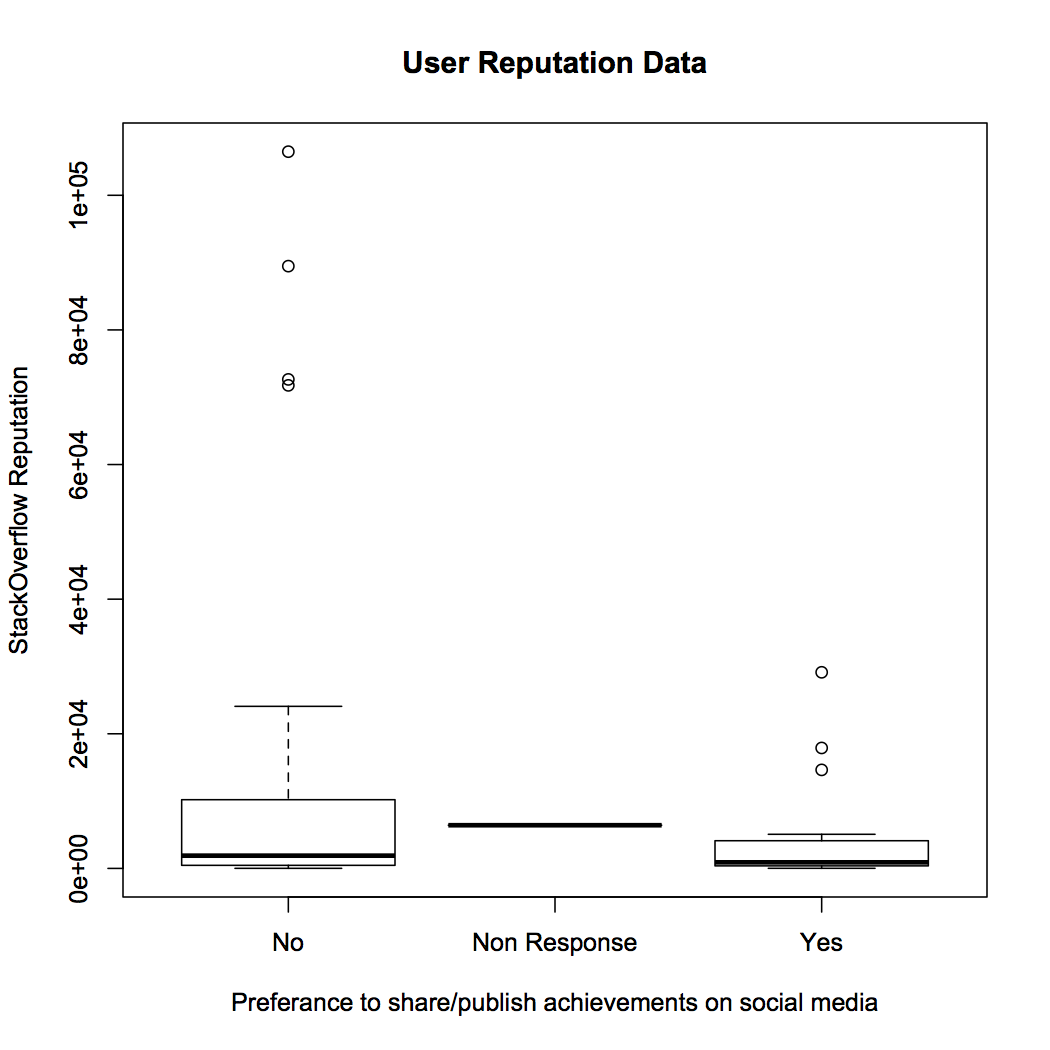
\includegraphics[scale=0.5]{figures/boxplot_reputation_compare_publish_reputation_bool.png} 

Having the interviews, a user from the reputation level 1,000-9,999 provided us an interesting justification for not sharing in GitHub: “GitHub in my opinion is the only popular place where you can really show your skills, so answering your question, sharing StackOverflow badges on GitHub would do nothing” and not sharing in LinkedIn: “LinkedIn is in my opinion a place where headhunters live , not a place to share your achievements because you don’t find a soulmate who appreciate your achievement“. The members who agreed to share their achievements on Social Media preferred LinkedIn (91\%), Twitter (78\%) and Facebook (56\%). The answer to the question how your contribution will be affected if StackOverflow start to share your reputation and badges? confirm the interest of the lowest reputation level to increase their motivation (100\%). On the other side, the other reputations levels would be motivated only with 25\% in average of the the responses. Overall, we did not find enough evidence that Social Media can improve the current gamification. In fact, it is the use of badges among those acclimated to the community seems a point of contention probably worth studying on its own. 

\textbf{RQ2.How does current gamification used by StackOverflow need to be improve in order to meet the user requirements?}

We found based on the discussion with our team that the current gamification can be improved in the SO community.The badges and reputation currently provided by SO are static and non-exportable to resumes or personal websites. We took a pragmatic decision to include this question on the survey to identify if there is a definite need to improve the gamification elements in SO community and if it is then how can it be improved further. To study the current gamification in SO, we included three important research questions: what is the motivation to contribute, how much satisfaction is there with the current gamification and how the member would like to improve the current gamification. 
From the analysis of the responses we found that the main motivations to contribute on SO can vary according to the reputation level of the member. For example, the lowest reputation level is more interested on increasing their knowledge through asking questions. The medium reputation levels are more appealing to contribute on SO when applying their experience while building reputation. On the other hand, the highest reputation level is more focused on applying experience while challenging themselves with unusual questions. One answer from an interview can clarify this aspect : “Only if the question is interesting and deep enough for me, I would consider answering it, if it is not interesting or deep enough for me, I am not saying I am a good programmer, it’s only my personal taste”
Surprisingly, when asking about how satisfied are the members with the current gamification, the lower reputation levels are more satisfied than the higher reputation levels. For example, the lower levels(0-9,10-99) are satisfied with the current gamification. On the other hand, the higher  reputation levels (100-999, 1,000-9,9999 and more than 10,000) are dissatisfied with the current gamification. These results suggest that new users are attracted for the current use of badges and reputation while users with more experience are not completely convinced with the system. An answer from our interviews can provide us more insight about this phenomenon: “If a fresh person wants to start participating, asking, answering, then yes I agree that badges would play an important role in incentivize participation, ...when a newcomer would pay attention to those gamifications objects because he would know how StackOverflow works, he would know by that time that badges mean nothing”
In overall, all reputation levels agreed with about 40\% responses to share reputation and badges on GitHub as a feature to increase the contributions in the community. In our interviews, we found the same relationship between SO and GitHub, but in the other way round: “sharing GitHub on StackOverflow would made, increase the incentive to motivation to answer or ask question if they see the GitHub profile”. Through the interviews we observed a sense of devalued reputation and value of badges in SO.

\textbf{How would users like to include their reputation and badges on social media?}

As the part of preliminary analysis of the research question, we found evidence of people wanting to include their reputation and badges from SO to social media \footnote{http://meta.stackexchange.com/questions/141300/how-can-i-share-my-stack-overflow-reputation-on-facebook}. Based on the discussion, we suggested few ways in which the reputation and badges can be included/exported on Social media. Our suggestion came from a careful discussion based on the usability and functionality. We suggested to separate the badges on programming language as the current badges interface does not provide enough information about in which domain or technical proficiency it was awarded for. The results show that lower reputation users agree to include programming language classification in the badges while higher reputation users do not. The higher reputation users seem to have more justifications about the nonconformity of the current gamification. An interview provided us with  a better insight about this: “the process of earning reputation should be like exponentially difficult . If you get at the level A and then you answer twice many questions after level A, you wouldn’t get twice reputation than you got before level A, it should be exponentially difficult, the curve should not be flat.”. We can identify a necessity of changing the means by which assignment of  badges and reputation among the different reputation levels takes place.


Another interesting aspect we discovered while conducting our interviews was this concept of a tutorial. Even though this does not relate to our research questions, the idea brings up further points about stimulating users to post. During the interview of a low reputation user, a main issue with a lack of posting was correlated to a lack of stimuli from SO. This user suggested a helpful tips or tutorial option in which SO would gently prompt users about the features of the website and help them learn the tools at their disposal while they can build up their reputation. This method of a tutorial which is not annoying but helpful in teaching users is the same approach that video games have been using in their tutorials. If SO could find the same balance of creating a tutorial that is helpful but not annoying like popular video games have in the past, this would dramatically increase the input from these low reputation users and could even teach the medium to high users a thing or two. This core aspect of gamification, a tutorial, would be another feature that SO could add to help newcomers learn the ropes of a challenging but ultimately rewarding online experience.

\section{Discussion}

After compiling the results from the survey and with much consideration to the interviews, we have isolated some trends that look to be significant. We found that our research questions did not cut deep enough into the issue of gamification on SO. From both the interviews and the survey, it became clear that newer users value the reputation much more then established users. 



After collecting all the data from our research we expect to have a better understanding of how gamification and social media affects StackOverflow and its users. To be more precise, we will look at how these game design elements such as badges and reputation points. We will be collecting data to make sure if the current gamification is working to prompt users to be more active and engaging. Based on our findings we will hope to add our own contributions which will improve this system. We will also be looking at how social media is impacting the user experience. Our expected contributions will be based on the data we collect and the answers to our research questions. We are looking to end this extensive study with concrete improvements to StackOverflow’s: gamification implementation, social media synergy and user interaction.



\section{Conclusions and Future Work}

After analyzing the results obtained from the survey and interviews, we are convinced there is a need to improve the current gamification elements SO operates with. 

The most important result from this study is that the gamification elements on SO are less effective at motivating acclimated users. Using a different mechanism for badge and reputation acquisition could potentially solve this. Further improvements to gamification in the kernel are needed before thinking on adding external features that would export the SO reputation system to other platforms. 

There is a definite need from the creators of SO to make the community impartial and unbiased so that even new users (without reputation) can contribute.  


% REFERENCES FORMAT
% References must be the same font size as other body text.
% \bibliographystyle{SIGCHI-Reference-Format}
% \bibliography{document}

\begin{thebibliography}{9}

\bibitem{Antin}
Antin, Judd, and Elizabeth F. Churchill. "Badges in social media: A social psychological perspective." CHI 2011 Gamification Workshop Proceedings (Vancouver, BC, Canada, 2011). 2011.

\bibitem{Bosu}
Bosu, Amiangshu, et al. "Building reputation in stackoverflow: an empirical investigation." Proceedings of the 10th Working Conference on Mining Software Repositories. IEEE Press, 2013.

\bibitem{Caponetto}
Caponetto, Ilaria, Jeffrey Earp, and Michela Ott. "Gamification and Education: A Literature Review." ECGBL2014-8th European Conference on Games Based Learning: ECGBL2014. Academic Conferences and Publishing International, 2014.

\bibitem{Cavusoglu}
Cavusoglu, Huseyin, Zhuolun Li, and Ke-Wei Huang. "Can Gamification Motivate Voluntary Contributions?: The Case of StackOverflow Q\&A Community." Proceedings of the 18th ACM Conference Companion on Computer Supported Cooperative Work \& Social Computing. ACM, 2015.

\bibitem{Deterding}
Deterding, Sebastian, et al. "Gamification. Using game-design elements in non-gaming contexts." CHI'11 Extended Abstracts on Human Factors in Computing Systems. ACM, 2011.

\bibitem{Easterbrook}
Easterbrook, Steve, et al. "Selecting empirical methods for software engineering research." Guide to advanced empirical software engineering. Springer London, 2008. 285-311.

\bibitem{Jin}
Jin, Yong, et al. "Quick Trigger on Stack Overflow: A Study of Gamification-influenced Member Tendencies." , 1916.

\bibitem{Marder}
Marder, Andrew. "Stack overflow badges and user behavior: an econometric approach." Proceedings of the 12th Working Conference on Mining Software Repositories. IEEE Press, 2015.

\bibitem{McGonigal}
McGonigal, Jane. "Reality is broken: Why games make us better and how they can change the world." Penguin, 2011.

\bibitem{Hägglund}
Hägglund, Per. "Taking gamification to the next level.", 2012.

\bibitem{Hamari}
Hamari, Juho, Jonna Koivisto, and Harri Sarsa. "Does gamification work?--a literature review of empirical studies on gamification." System Sciences (HICSS), 2014 47th Hawaii International Conference on. IEEE, 2014.

\bibitem{Rughinis}
Rughinis, Razvan. "Gamification for productive interaction: Reading and working with the gamification debate in education." Information Systems and Technologies (CISTI), 2013 8th Iberian Conference on. IEEE, 2013.

\bibitem{Ryan}
Ryan, Richard M., C. Scott Rigby, and Andrew Przybylski. "The motivational pull of video games: A self-determination theory approach." Motivation and emotion 30.4 (2006): 344-360.

\bibitem{Slag}
Slag, Rogier, Mike de Waard, and Alberto Bacchelli. "One-day flies on StackOverflow."

\bibitem{Vasilescu}
Vasilescu, Bogdan, Vladimir Filkov, and Alexander Serebrenik. "StackOverflow and GitHub: associations between software development and crowdsourced knowledge." Social Computing (SocialCom), 2013 International Conference on. IEEE, 2013.

\bibitem{Wang}
Wang, Shaowei, David Lo, and Lingxiao Jiang. "An empirical study on developer interactions in StackOverflow." Proceedings of the 28th Annual ACM Symposium on Applied Computing. ACM, 2013.


\end{thebibliography}

\end{document}

%%% Local Variables:
%%% mode: latex
%%% TeX-master: t
%%% End:
